\documentclass[10pt]{article}
%%%%%%%%%%%%%%% Define following before importing preamble
\def\Type{LessonCaelan}
\def\TypeNum{Lesson 4}
\def\TypeTitle{Limits at Infinity\\Key}
\def\Semester{Fall 2021} %Not Used 
\def\Course{MATH 1190 \& 1210}
\def\Targets{ {\target{L2}}, {\target{L2}} }

%%%%%%%%%%%%%%%Preamble must come after above%%%%%%%
\usepackage{preambleDJ}



%%%%%%%%%%%% BEGIN DOCUMENT %%%%%%%%%%%%%%%
%%%%%%%%%%%% BEGIN DOCUMENT %%%%%%%%%%%%%%%
%%%%%%%%%%%% BEGIN DOCUMENT %%%%%%%%%%%%%%%
%%%%%%%%%%%% BEGIN DOCUMENT %%%%%%%%%%%%%%%
%%%%%%%%%%%% BEGIN DOCUMENT %%%%%%%%%%%%%%%

\begin{document}

\pagestyle{otherpages}
\thispagestyle{firstpage}
\vs{.5}

\textbf{Intended Learning Outcomes}
After this lesson, you will be able to 

\begin{itemize}
    \item Identify the form of a limit. (\target{L2})
    \item Identify the method to use to evaluate a limit based on its form. (\target{L2})
    \item Evaluate a limit based on its form. (\target{L2})
\end{itemize}

\vspace{-0.5cm}

\hrulefill
~\\
\blue{\bf Rust-Remover Warm-up: Exponent Properties} This exercise helps ``knock the rust off" of some exponent properties that we will be using today.\\
\def\sz{.2}
{\large
\noindent\makebox[\linewidth][s]{$\ds \bullet\, x^{-p}=\frac{1}{x^p} \hs{\sz} \bullet\,\frac{1}{x^{-q}}=\frac{x^q}{1}=x^q \hs{\sz} \bullet\, \frac{x^m}{x^n}=\frac{x^{m-n}}{1}=x^{m-n} \hs{\sz} \bullet\,  \frac{x^m}{x^n}=\frac{1}{x^{n-m}} \hs{\sz} \bullet\,   (x^a)^b=x^{a\cdot b} \hs{\sz} \bullet\,  \sqrt[b]{x}=x^\frac{1}{b}$}
}

\enum{
\item Work together at your tables to re-write each expression with only positive exponents. Note that $e$ is a constant: $e\approx2.71828182846\dots$.
\tasksA{4}{
\task $\ds x^{-4}=$\unline{.5}{  \blue{$\ds \frac{1}{x^4}$}  }{.3}
\task $\ds \frac{4}{7x^{-6}}=$\unline{.5}{\blue{$\ds \frac{4x^6}{7}$} }{.3}
\task  $\ds  \frac{10x^{-3}}{x^4}=\unlineb{.5}{\ds \frac{10}{x^7}}{.25}$\\
\sol{\al{  \frac{10x^{-3}}{x^4} &=\frac{10}{x^4\cdot x^3}\\=\frac{10}{x^{4+3}}&=\frac{10}{x^7} }}
\task $\ds \frac{3e^{-2x}}{5x^{-4}}=$\unline{.5}{\blue{$\ds \frac{3x^4}{5e^{2x}}$}  }{.3}
}
\vs{-.4}
\item Work together at your tables to re-write each expression using exponent notation. All terms with exponents should be in the numerator (negative exponents are ok).
\tasksA{4}{
\task $\ds \sqrt[4]{x}=$\unline{.5}{ \blue{$\ds x^{\frac{1}{4}}$} }{.3}
\task  $\ds \sqrt[4]{x^3}=$\unline{.5}{    \blue{$\ds (x^3)^{\frac{1}{4}}=x^{\frac{3}{4}}$} }{.3}
\task  $\ds \frac{1}{\sqrt[4]{x^3+1}}=$\unline{.5}{\hs{-0}\blue{$\ds (x^3+1)^{-\frac{1}{4}}$} }{.3}
\sol{
\al{
\frac{1}{\sqrt[4]{x^3+1}}&=\frac{1}{(x^3+1)^{1/4}}\\
&=(x^3+1)^{-\frac{1}{4}}
}
}
\task   $\ds \frac{7x^2}{\sqrt{x^3}}=\unlineb{.5}{7x^{1/2}}{.25}$ \\
%\task  $\ds \frac{7}{\sqrt{x^3}}=$\unline{.5}{ \blue{$\ds 7x^{-\frac{3}{2}}$} }{.3}\\
\sol{
\al{
\frac{7x^2}{\sqrt{x^3}}&=\frac{7x^{2}}{(x^3)^{1/2}}\\
&=\frac{7^{4/2}}{x^{3/2}}\\
&=7x^{\frac{4}{2}-\frac{3}{2}}\\
&=7x^{1/2}
}
}
}
}
\vs{-.4}
\bluebf{Warm-up} \exercise{\target L2} Last time, we talked about evaluating limits using the Main Continuity Theorem.  For each of the limits below, decide if it can be evaluated using the Main Continuity Theorem. If so, explain why and find the limit. If not, explain why not.
\tasksE{3}{
\task $\ds \lim_{x\to 1^-}\frac{1}{x-1}$
\sol{
$x=1$ is not in the domain since we have a division by $0$: $\ds \frac{1}{1-1}=\frac{1}{0}$. Therefore we cannot use the M.C.T. to evaluate the limit. We will see later in today's lesson how to handle this situation.

}
\task  $\ds \lim_{x\to 2}\frac{1}{x-1}$
\sol{
$x=2$ {\em is} in the domain since we do not have a division by $0$, square root of a negative number, nor log of $0$ or a negative number. Therefore by the M.C.T., \\$\ds \lim_{x\to 2}\frac{1}{x-1}=\frac{1}{2-1}=\frac{1}{1}=1$.
}
\task $\ds \lim_{x\to \infty}\frac{1}{x-1}$
\sol{
The M.C.T. assumes we are finding a limit to a finite number $a$: $\ds \lim_{x\to a}\frac{1}{x-1}$. Since $\infty$ is not a finite number, we cannot use the M.C.T. We will see later in today's lesson how to handle this situation.
}
}

 \newpage
\newpage
{\bf\color{blue}Warm-up Exercise 1.} Four graphs are given below.\\

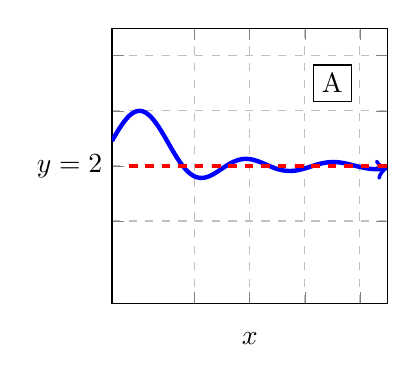
\begin{tikzpicture}[scale=1]
          \begin{axis}[
        %    axis y line = left,
        %    axis x line = bottom,
            xlabel={$x$},
            xtick       = {1,2,3,4},
            xticklabels = {},
            ytick       = {1,2,3,4},
            yticklabels = {,\red{$y=2$},,},
            samples     = 160,
            domain      = -1:4.5,
            restrict y to domain=-1:4.5,
            xmin = -0.5, xmax = 4.5,
            ymin = -0.5, ymax = 4.5,
            grid=both, grid style=dashed,
            width=2in, height=2in
          ]
          % pieces 1 and 2
          \addplot[domain=-0.5:4.5, blue, ultra thick, ->] {2+sin(4*deg(x))/4/x};
                    \addplot[dashed, domain=-0.2:4.5, red, ultra thick, -] {2};
          \node at (3.5,3.5) {\fbox{A}};
        \end{axis}
    \end{tikzpicture}
%
\hfill
%
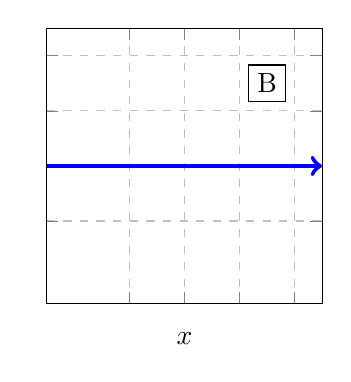
\begin{tikzpicture}[scale=1]
          \begin{axis}[
        %    axis y line = left,
        %    axis x line = bottom,
            xlabel={$x$},
            xtick       = {1,2,3,4},
            xticklabels = {},
            ytick       = {1,2,3,4},
            yticklabels = {},
            samples     = 160,
            domain      = -1:4.5,
            restrict y to domain=-1:4.5,
            xmin = -0.5, xmax = 4.5,
            ymin = -0.5, ymax = 4.5,
            grid=both, grid style=dashed,
            width=2in, height=2in
          ]
          % pieces 1 and 2
          \addplot[domain=-0.5:4.5, blue, ultra thick, ->] {2};
          \node at (3.5,3.5) {\fbox{B}};
        \end{axis}
    \end{tikzpicture}
%
\hfill
%
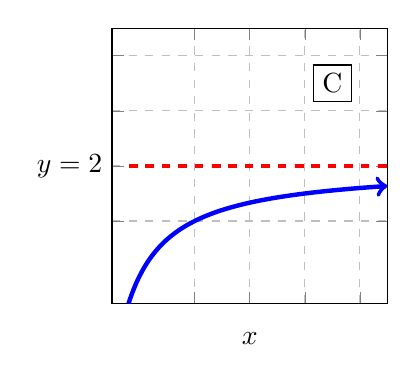
\begin{tikzpicture}[scale=1]
          \begin{axis}[
        %    axis y line = left,
        %    axis x line = bottom,
            xlabel={$x$},
            xtick       = {1,2,3,4},
            xticklabels = {},
            ytick       = {1,2,3,4},
            yticklabels = {,\red{$y=2$},,},
            samples     = 160,
            domain      = -1:4.5,
            restrict y to domain=-1:4.5,
            xmin = -0.5, xmax = 4.5,
            ymin = -0.5, ymax = 4.5,
            grid=both, grid style=dashed,
            width=2in, height=2in
          ]
          % pieces 1 and 2
          \addplot[domain=-0.2:4.5, blue, ultra thick, ->] {2-2/(x+1)};
          \addplot[dashed, domain=-0.2:4.5, red, ultra thick, -] {2};
          \node at (3.5,3.5) {\fbox{C}};
        \end{axis}
    \end{tikzpicture}
%
\hfill
%
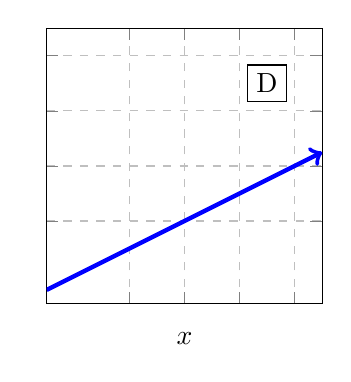
\begin{tikzpicture}[scale=1]
          \begin{axis}[
        %    axis y line = left,
        %    axis x line = bottom,
            xlabel={$x$},
            xtick       = {1,2,3,4},
            xticklabels = {},
            ytick       = {1,2,3,4},
            yticklabels = {},
            samples     = 160,
            domain      = -1:4.5,
            restrict y to domain=-1:4.5,
            xmin = -0.5, xmax = 4.5,
            ymin = -0.5, ymax = 4.5,
            grid=both, grid style=dashed,
            width=2in, height=2in
          ]
          % pieces 1 and 2
          \addplot[domain=-0.5:4.5, blue, ultra thick, ->] {0.5*x};
          \node at (3.5,3.5) {\fbox{D}};
        \end{axis}
    \end{tikzpicture}
\nti{
For each graph, students will have to make assumptions about the behavior of the graph as $x\to \infty$. I will tell my class to ask themselves ``What do you think happens to the graph beyond what we can see? How would you describe this?"  \\
\mpageT{.25}{.25}[\hs{.1}]{
Amplitude of oscillations (i.e. ``wobbles" or ``bumps") seem to be decreasing. If we assume this will continue, then graph continues to approach $y=2$ (see red dashed line) as $x\to\infty$. To the limit exists and $\displaystyle\lim_{x\to\infty}f(x)=2$. 
}{
The graph appears to start and stay on $y=2$. If we assume this behavior continues, then the limit exists and $\displaystyle\lim_{x\to\infty}f(x)=2$. 
}
\hs{.1}
\mpageT{.22}{.22}[\hs{.1}]{
The graph appears to be increasing to an asymptote at $y=2$ (see red dashed line on graph). If we assume this trend continues, then the limit exists and $\displaystyle\lim_{x\to\infty}f(x)=2$.  }{
It appears that the graph is headed up and to the right. If we assume this trend continues, then the $y$-values will continue to get larger and therefore $\displaystyle\lim_{x\to\infty}f(x)=\infty$ (i.e. DNE). }
}
For each statement below, decide which of the graphs appears to satisfy the statement. Specify all applicable answers.
\begin{enumerate}
\item[(a)] $\displaystyle\lim_{x\to\infty}f(x)=2$ \dotfill \unline{1.5}{\blue{A, B, C}}{.25}\\
\item[(b)] $\displaystyle\lim_{x\to\infty}f(x)$ exists \dotfill \unline{1.5}{\blue{A, B, C}}{.25}\\
\item[(c)] $\displaystyle\lim_{x\to\infty}f(x)$ DNE\dotfill  \unline{1.5}{\blue{D.  Graph keeps increasing to $\infty$.}}{.25}\\
\end{enumerate}

%\newpage
\mpageT{.75}{.25}[\hs{.1}]{
\minil {\it Functions with Infinite Limits at Infinity}\\
%{\em Exponentials \hfill Power Functions \hfill Logarithms}
\mpageTth{.32}{.33}{.32}{\centering
{\em Exponentials}\\
\blue{
Examples: $e^x$, $2^x$, $7^x$. Exponentials are all of form $a^x$: 
$$a^x\rightarrow \infty$$ when $a>1$.
}
}{\centering
{\em Power Functions }\\
\blue{
Examples: $x^2$, $x^{1/2}$, $x^7$, $x^{1/3}$. Power functions of form $x^n$.
$$x^n\rightarrow \infty$$ when $n>0$.
}
}{\centering
{\em Logarithms}
\blue{
Examples: $\ln(x)$, $\log_{10}(x)$, $\log_2(x)$.
Logarithms of form $\log_a(x)$
$$\log_a(x)\rightarrow \infty$$ when $a>1$.
}
}
}{
    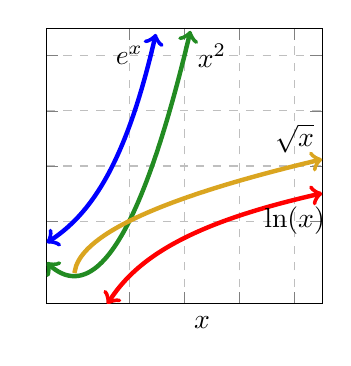
\begin{tikzpicture}[scale=1]
          \begin{axis}[
        %    axis y line = left,
        %    axis x line = bottom,
            xlabel={$x$},
            xtick       = {1,2,3,4},
            xticklabels = {},
            ytick       = {1,2,3,4},
            yticklabels = {},
            xlabel style={anchor=west},
            ylabel style={anchor=south},
            samples     = 160,
            domain      = -1:4.5,
            restrict y to domain=-1:4.5,
            xmin = -0.5, xmax = 4.5,
            ymin = -0.5, ymax = 4.5,
            grid=both, grid style=dashed,
            width=2in, height=2in
          ]
          % pieces 1 and 2
          \addplot[domain=-0.5:4.5, blue, ultra thick, <->] {e^x};
          \node at (2.5,4) {$x^2$};
          \addplot[domain=-0.5:4.5, ForestGreen, ultra thick, <->] {x^2};
          \node at (1,4) {$e^x$};
          \addplot[domain=-0.5:4.5, Goldenrod, ultra thick, ->] {x^(1/2)};
          \node at (4,2.5) {$\sqrt{x}$};
          \addplot[domain=0.6:4.5, red, ultra thick, <->] {ln(x)};
          \node at (4,1) {$\ln(x)$};
        \end{axis}
    \end{tikzpicture}
}
\\

\newpage 
\lform   \blue{  \bf$\dfrac{c}{\infty}$} 


\exercise{\target{L2}} Use your knowledge of numbers and fractions to select an appropriate answer choice for the question below. If you aren't sure how to answer, then try to come up with some fractions in which the given situations occur to help you to form a guess.\\

When the {\it denominator} of a fraction grows ever larger without bound - all other things held constant - the value of the fraction...\\
\mpageT{.5}{.5}{
    \begin{enumerate}
    \item[A.] \blue{approaches $0$. See work in pre-class activity.}
    \item[B.] becomes larger.
    \item[C.] becomes larger without bound.
    \item[D.] could become larger, approach $0$, or anything in between based on the given information.
    \end{enumerate}
    }{
   \blue{  Here's one way to illustrate the idea behind Form $\dfrac{c}{\infty}$.
$$
%\definecolor{Gray}{gray}{0.7}
%\newcolumntype{g}{>{\columncolor{Gray}}c}
\begin{array}{c |c|c|c|c}
 x&1&10&100&1000  \\ \hline
3/x&3&0.3&0.03&0.003
\end{array}
$$
}
}
    

%%%%%%%%%

%%%%%%%%%

\example{\target{L2}} Find the following limits using forms: \\
\mpageTth{.33}{.35}{.33}{
$\displaystyle\lim_{x\to\infty} \frac{1}{x^5}=$ \unline{.5}{\blue{0}}{.25}\\
\blue{
Since $x^5 \rightarrow \infty$ we have\\
Form $\dfrac{1}{\infty}$. We know this \\approaches $0$.
}
}{
$\displaystyle\lim_{x\to\infty} \frac{10}{\log_4(x)+\sqrt{x-4}}=$ \unline{.5}{\blue{0}}{.25}\\
\blue{
Since $\log_4(x)\to \infty$ and \\
$(x-4)^{1/2}\to \infty$,  denominator \\
approaches $\infty$. \\Form is $\dfrac{10}{\infty}$ which \\approaches $0$.
}
}{
$\displaystyle\lim_{x\to\infty} 6e^{-x}=$ \unline{.5}{\blue{0}}{.25}\\
\blue{
$6e^{-x}=\dfrac{6}{e^x}$. Since $e^x\to \infty$, Form is $\dfrac{6}{\infty}$ which approaches $0$.
}
}
\vfill

\exercise{\target{L2}} Find the following limits using forms. (Practice showing your work, even if you know the answer!) \vs{-.2}\\
\mpageTth{.33}{.33}{.33}{
$\displaystyle\lim_{x\to\infty} 5x^{-3}=$ \unline{.5}{\blue{0}}{.25}\\
\blue{
$5x^{-3}=\dfrac{5}{x^3}$. $x^3\to\infty$ \\Form is $\dfrac{5}{\infty}$ which \\approaches $0$.
}
}{
$\displaystyle\lim_{x\to\infty} -\frac{1}{e^x+x^{1000}}=$ \unline{.5}{\blue{0}}{.25}\\
\blue{
Both $e^x\to \infty$ and \\$x^{1000}\to \infty$ so $e^x+x^{1000}\to \infty$. \\Form is $\dfrac{1}{\infty}$ which \\approaches $0$.
}
}{
$\displaystyle\lim_{x\to\infty} \frac{e^{-x}}{x^2} =$ \unline{.5}{\blue{0}}{.25}\\
\blue{
$\dfrac{e^{-x}}{x^2}=\dfrac{1}{e^{x}\cdot x^2}$.  Both $e^x\to\infty$ and $x^2\to\infty$. Thus $e^x \cdot x^2\to \infty$ and Form is $\dfrac{1}{\infty}$ which approaches $0$.
}
}

\vfill
\newpage

\lform  \blue{\bf $\dfrac{\infty}{c}$ }


\exercise{\target{L2}} Use your knowledge of numbers and fractions to select an appropriate answer choice for the question below. If you aren't sure how to answer, then try to come up with some fractions in which the given situations occur to help you to form a guess.\\

When the {\it numerator} of a fraction grows ever larger without bound - all other things held constant - the value of the fraction...\\
\mpageT{.5}{.5}{
    \begin{enumerate}
    \item[A.] approaches $0$.
    \item[B.] becomes larger.
    \item[C.] \blue{becomes larger without bound. See pre-class work. }
    \item[D.] could become larger, approach $0$, or anything in between based on the given information.
    \end{enumerate}
}{
\blue{
 Here's one way to illustrate the idea behind Form $\dfrac{\infty}{c}$.
$$
%\definecolor{Gray}{gray}{0.7}
%\newcolumntype{g}{>{\columncolor{Gray}}c}
\begin{array}{c |c|c|c|c}
 x&1&10&100&1000  \\ \hline
x/3&1/3&10/3&100/3&1000/3
\end{array}
$$
}
}\vs{.1}\\ 
\example{\target{L2}} Find the following limits using forms:\vs{-.2}\\
\mpageTth{.33}{.33}{.33}{
$\displaystyle\lim_{x\to\infty} \frac{e^x+1}{2}=$ \unline{.5}{\blue{$\infty$} }{.25}\\
\blue{
$e^x+1\to \infty$ so Form is $\dfrac{\infty}{2}$ \\which approaches $\infty$.
}
}{
$\displaystyle\lim_{x\to\infty} \frac{-2x^2}{3\sqrt[4]{x}}=$ \unline{.5}{\blue{-$\infty$}}{.25}\\
\blue{
$\dfrac{-2x^2}{3\sqrt[4]{x}}=\dfrac{-2x^2}{3x^{1/4}}\\
=\dfrac{-2x^2\cdot x^{-1/4}}{3}=\dfrac{-2x^{2-1/4}}{3}\\
=\dfrac{-2x^{7/4}}{3}$.  $-2x^{7/4}\to -\infty$ so Form is $\dfrac{-\infty}{3}$ which approaches $-\infty$. 
}
}{
$\displaystyle\lim_{x\to\infty} \frac{1-\ln(x)}{-3}=$ \unline{.5}{\blue{$\infty$}}{.25} \\
\blue{
$\ln(x)\to\infty$ so $1-\ln(x)\to -\infty$.  Form is $\dfrac{-\infty}{-3}$ which approaches $+\infty$.
}
}
\exercise{\target{L2}} Find the following limits using forms. (Practice showing your work, even if you know the answer!)\vs{-.2}\\
\mpageTth{.33}{.33}{.33}{
$\displaystyle\lim_{x\to\infty} -\frac{\sqrt{x}}{5}=$ \unline{.5}{ \blue{-$\infty$} }{.25}\\
\blue{
$\sqrt{x}\to \infty$ so Form is $-\dfrac{\infty}{5}$ \\
which approaches $-\infty$.
}
}{
$\displaystyle\lim_{x\to\infty} \frac{x^5}{2x}=$ \unline{.5}{ \blue{$\infty$} }{.25}\\
\blue{
$\dfrac{x^5}{2x}=\dfrac{x^4}{2}$. Since $x^4\to\infty$ \\
Form is $\dfrac{\infty}{2}$ which \\approaches $\infty$.
}
}{ 
$\displaystyle\lim_{x\to\infty} \frac{1}{2e^{-x}}=$ \unline{.5}{ \blue{$\infty$} }{.25}\\
\blue{
$\dfrac{1}{2e^{-x}}=\dfrac{e^x}{2}$.  Since $e^x\to\infty$ Form is $\dfrac{\infty}{2}$ which approaches $\infty$.
}
}



%%%%%%%%%
\newpage%
%%%%%%%%%
%$\left({\it \text{\bf \blue{Form} }\dfrac{\infty}{\infty}}\right)$
\lform  \blue{\bf $\dfrac{\infty}{\infty}$}


\exercise{\target{L2}} Use your knowledge of numbers and fractions to select an appropriate answer choice for the question below. If you aren't sure how to answer, then try to come up with some fractions in which the given situations occur to help you to form a guess.\\

When both the {\it numerator and denominator} grow ever larger without bound, the value of the fraction...\\
\mpageT{.5}{.5}{
    \begin{enumerate}
    \item[A.] approaches $0$.
    \item[B.] becomes larger.
    \item[C.] becomes larger without bound.
    \item[D.] \blue{could become larger, approach $0$, or anything in between based on the given information.}
    \end{enumerate}
}{
}\\
%%%

\mpageT{.75}{.25}[\hs{.1}]{
{\bf\color{blue}Mini-lecture. } {\it Functions with Infinite Limits at Infinity}
%{\em Exponentials \hfill Power Functions \hfill Logarithms}
\mpageTth{.32}{.33}{.32}[\hs{.1}][\hs{.1}]{{\centering
{\em Exponentials}}\\
\blue{
Exponential functions such as $e^x$ grow much faster than other functions we will see. The general form is $a^x$ where $a>1$.
}
}{{\centering
{\em Power Functions }}\\
\blue{
Power functions such as $x^2$ or $x^{1/2}$ grow much faster than logarithmic functions. The general form is $x^n$ where $n>0$. {\em Within power functions}, larger exponents mean faster growth.
}
}{{\centering
{\em Logarithms}}\\
\blue{
Slowest growing.
}
}
}{
    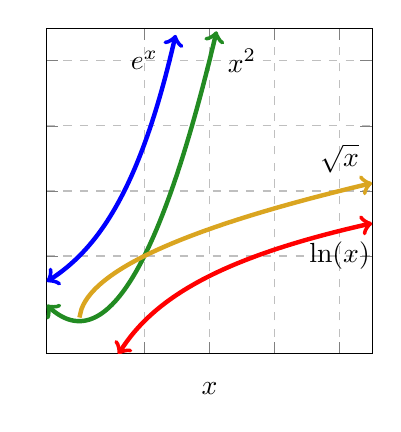
\begin{tikzpicture}[scale=1]
          \begin{axis}[
        %    axis y line = left,
        %    axis x line = bottom,
            xlabel={$x$},
            xtick       = {1,2,3,4},
            xticklabels = {},
            ytick       = {1,2,3,4},
            yticklabels = {},
            samples     = 160,
            domain      = -1:4.5,
            restrict y to domain=-1:4.5,
            xmin = -0.5, xmax = 4.5,
            ymin = -0.5, ymax = 4.5,
            grid=both, grid style=dashed,
            width=2.25in, height=2.25in
          ]
          % pieces 1 and 2
          \addplot[domain=-0.5:4.5, blue, ultra thick, <->] {e^x};
          \node at (2.5,4) {$x^2$};
          \addplot[domain=-0.5:4.5, ForestGreen, ultra thick, <->] {x^2};
          \node at (1,4) {$e^x$};
          \addplot[domain=-0.5:4.5, Goldenrod, ultra thick, ->] {x^(1/2)};
          \node at (4,2.5) {$\sqrt{x}$};
          \addplot[domain=0.6:4.5, red, ultra thick, <->] {ln(x)};
          \node at (4,1) {$\ln(x)$};
        \end{axis}
    \end{tikzpicture}
}
{\em Key Idea for Form $\dfrac{\infty}{\infty}$}\\
\blue{We're going to choose the Dominant Term (i.e. the fastest growing) in both the numerator and denominator to create a new fraction. This new fraction will have the same limit as our original.} \\\\
\example{\target{L2}} Find the following limits using forms:\\
\mpageTth{.33}{.33}{.36}[\hs{.15}][\hs{.15}]{
$\displaystyle\lim_{x\to\infty} \frac{\log_2(x)}{x^3+4x-1}=$ \unline{.5}{ \blue{$0$} }{.25}\\
\blue{
\itemC{
\item Dominant term in numerator: $\log_2(x)$\\
\item Dominant term in denominator: $x^3$.\\
\item $\ds \lim_{x\to\infty} \frac{\log_2(x)}{x^3+4x-1} $\\
$\ds \qquad \qquad \sim \lim_{x\to\infty} \frac{\log_2(x)}{x^3}$\\
\item Form is $\dfrac{\infty}{\infty}$ with\\ 
$\dfrac{slower}{much\,\, faster}\to 0$. \\
\item Thus $\ds \lim_{x\to\infty} \frac{\log_2(x)}{x^3}=0$\\
$\ds \Rightarrow \lim_{x\to\infty} \frac{\log_2(x)}{x^3+4x-1}=0$
}
}
}{
$\displaystyle\lim_{x\to\infty} \frac{4^x+\ln(x)}{1-\sqrt[3]{x}}=$ \unline{.5}{ \blue{$-\infty$} }{.25} \\
\blue{
\itemC{
\item Dominant term in numerator: $4^x$\\
\item Dominant term in denominator: $-\sqrt[3]{x}=-x^{1/3}$.\\
\item $\ds \lim_{x\to\infty} \frac{4^x+\ln(x)}{1-\sqrt[3]{x}} \sim \lim_{x\to\infty} \frac{4^x}{-x^{1/3}}$\\
\item Form is $\dfrac{\infty}{-\infty}$ with\\ 
$\dfrac{much\,\,faster}{-slower}\to -\infty$.\\
\item Thus $\ds \lim_{x\to\infty} \frac{4^x}{-x^{1/3}}=-\infty$\\
$\ds \Rightarrow \lim_{x\to\infty} \frac{4^x+\ln(x)}{1-\sqrt[3]{x}} =-\infty$
}
}
}{
$\displaystyle\lim_{x\to\infty} \frac{\log_2(x)-\sqrt{x}}{2\sqrt{x+5}-4}=$ \unline{.5}{ \blue{$-\dfrac{1}{2}$} }{.25}\\
\blue{
\itemC{
\item Dominant term in numerator: $-\sqrt{x}$
\item Dominant term in denominator: $2\sqrt{x}$. (The ``$+5$" portion of $2\sqrt{x+5}$ is not growing).
\item $\ds \lim_{x\to\infty} \frac{\log_2(x)-\sqrt{x}}{2\sqrt{x+5}-4} \sim \lim_{x\to\infty} \frac{-\sqrt{x}}{2\sqrt{x}}$\\
$\ds =\lim_{x\to \infty} \frac{-1}{2}=-\frac{1}{2}$
\item Thus $\ds \lim_{x\to\infty} \frac{-\sqrt{x}}{2\sqrt{x}}=-\frac{1}{2}$\\
$\ds \Rightarrow \lim_{x\to\infty} \frac{\log_2(x)-\sqrt{x}}{2\sqrt{x+5}-4}=-\frac{1}{2}$
}
}
}


\newpage
\exercise{\target{L2}} Find the following limits using forms. (Practice showing your work, even if you  know the answer!)\\
\mpageTth{.33}{.35}{.36}[\hs{.15}][\hs{.15}]{
$\displaystyle\lim_{x\to\infty} \frac{7^x-x}{x^7}=$ \unline{.5}{ \blue{$\infty$}}{.25}\\
\blue{
\itemC{
\item Dominant term in numerator: $7^x$
\item Dominant term in denominator: $x^7$.
\item $\ds \lim_{x\to\infty} \frac{7^x-x}{x^7}\sim \lim_{x\to\infty} \frac{7^x}{x^7}$
\item Form is $\dfrac{\infty}{\infty}$ with\\ 
$\dfrac{much \,\,faster}{slower}\to \infty$. 
\item Thus $\ds \lim_{x\to\infty} \frac{7^x}{x^7}=\infty$\\
$\ds \Rightarrow  \lim_{x\to\infty} \frac{7^x-x}{x^7}=\infty$
}
}
}{
$\displaystyle\lim_{x\to\infty} \frac{\sqrt{x+1}}{4-x-\ln(x)}=$ \unline{.5}{ \blue{$0$}}{.25}\\
\blue{
\itemC{
\item Dominant term in numerator: $\sqrt{x}$. (The ``$+1$" is not growing)
\item Dominant term in denominator: $-x$.
\item $\ds \lim_{x\to\infty} \frac{\sqrt{x+1}}{4-x-\ln(x)}\sim \lim_{x\to\infty} \frac{\sqrt{x}}{-x}$
\item This simplifies further:\\
$$\ds \lim_{x\to\infty} \frac{x^{1/2}}{-x}=\frac{1}{-x^{1/2}}$$
\item Form $\dfrac{1}{-\infty}$ which approaches $0$.
\item $\ds \lim_{x\to\infty} \frac{\sqrt{x}}{-x}=0$\\
$\ds \Rightarrow \lim_{x\to\infty} \frac{\sqrt{x+1}}{4-x-\ln(x)}=0$
}
}
}{
$\displaystyle\lim_{x\to\infty} \frac{\sqrt{x^2+1}}{4-3x-\ln(x)}=$ \unline{.5}{ \blue{$\ds -\frac{1}{3}$} }{.25}\\
\blue{
\itemC{
\item Dominant term in numerator: $\sqrt{x^2}$. (The ``$+1$" is not growing)
\item Dominant term in denominator: $-3x$.
\item $\ds \lim_{x\to\infty} \frac{\sqrt{x^2+1}}{4-3x-\ln(x)} \sim \lim_{x\to\infty} \frac{\sqrt{x^2}}{-3x}$
\item This simplifies:\\
$$\lim_{x\to\infty} \frac{\sqrt{x^2}}{-3x}=\lim_{x\to\infty} \frac{x}{-3x}=\lim_{x\to\infty}\frac{1}{-3}=-\frac{1}{3}$$
($\sqrt{x^2}=x$ for $x>0$)
\item $\ds  \lim_{x\to\infty} \frac{\sqrt{x^2}}{-3x}=-\frac{1}{3}$\\
$\ds \Rightarrow \lim_{x\to\infty} \frac{\sqrt{x^2+1}}{4-3x-\ln(x)}=-\frac{1}{3}$
}
}
}

\mpageTth{.33}{.33}{.36}[\hs{.15}][\hs{.15}]{
$\displaystyle\lim_{x\to\infty} \frac{1000-x^{1000}}{x^e-e^x}=$ \unline{.5}{ \blue{$0$}}{.25}\\
\blue{
\itemC{
\item Dominant term in numerator: $-x^{1000}$. 
\item Dominant term in denominator: $-e^x$.
\item $\ds \lim_{x\to\infty} \frac{1000-x^{1000}}{x^e-e^x} \\$
$\ds \qquad \sim \lim_{x\to\infty} \frac{-x^{1000}}{-e^x}$
\item \item Form is $\dfrac{\infty}{\infty}$ with\\ 
$\dfrac{slower}{much \,\,faster}\to 0$. 
\item $\ds \lim_{x\to\infty} \frac{-x^{1000}}{-e^x}=0$\\
$\ds \Rightarrow \lim_{x\to\infty} \frac{1000-x^{1000}}{x^e-e^x}=0$
}
}
}{
$\displaystyle\lim_{x\to\infty} \frac{5e^{2x}+3e^x+1}{e^{2x}-5e^x+6}=$ \unline{.5}{ \blue{$5$}}{.25} \\
\blue{
\itemC{
\item Dominant term in numerator: $5e^{2x}$. 
\item Dominant term in denominator: $e^{2x}$.
\item $\ds \lim_{x\to\infty} \frac{5e^{2x}+3e^x+1}{e^{2x}-5e^x+6} $\\
$\ds \qquad \qquad \sim \lim_{x\to\infty} \frac{5e^{2x}}{e^{2x}}$
\item This simplifies further:
$$\lim_{x\to\infty} \frac{5e^{2x}}{e^{2x}}=\lim_{x\to\infty} \frac{5}{1}=5$$
\item $\ds \lim_{x\to\infty} \frac{5e^{2x}}{e^{2x}}=5$\\
$\ds \Rightarrow \lim_{x\to\infty} \frac{5e^{2x}+3e^x+1}{e^{2x}-5e^x+6}=5$
}
}
}{
%$\displaystyle\lim_{x\to\infty} \frac{x^5 +3x+\ln(x)}{2x+3}=$ \unline{.5}{}{.25} \\
\blue{
%
}
}
\vs{.5}~\\
\blue{\bf Summary of Limit Form   $\dfrac{\infty}{\infty}$}
After choosing dominant terms in numerator and denominator....
\itemI{
\item $\ds \frac{\text{much faster}}{\text{slower}}\to$ \blue{$\ds \pm \infty$}
\vs{.25}
\item $\ds \frac{\text{slower}}{\text{much faster}}\to$  \blue{$0$}
\vs{.25}
\item $\ds \frac{\text{about the same}}{\text{about the same}}\to$  \blue{Do some algebra to see if limit simplifies to another form.}
}

%%%%%%%%%

%%%%%%%%%
\newpage
%$\left({\it \text{\bf \blue{Form} }\dfrac{c}{0}}\right)$
\lform $\blue{\bf \dfrac{c}{0}}$



\exercise{\target{L2}}  Use your knowledge of numbers and fractions to select an appropriate answer choice for the question below. If you aren't sure how to answer, then try to come up with some fractions in which the given situations occur to help you to form a guess.\\

When the {\it denominator} of a fraction grows ever smaller - approaching $0$ - with all other things held constant, the value of the fraction...\\
\mpageT{.5}{.5}{
    \begin{enumerate}
    \item[A.] approaches $0$.
    \item[B.] becomes larger.
    \item[C.] \blue{becomes larger without bound.}
    \item[D.] could become larger, approach $0$, or anything in between based on the given information.
    \end{enumerate}
}{
\blue{ Here's one way to illustrate the idea behind Form $\dfrac{c}{0}$.
$$
%\definecolor{Gray}{gray}{0.7}
%\newcolumntype{g}{>{\columncolor{Gray}}c}
\begin{array}{c |c|c|c|c}
 x&1&1/10&1/100&1/1000  \\ \hline
3/x&3&30&300&3000
\end{array}
$$
}
}
\vs{.1}\\
\minil What can be said about a limit if we know its form resembles $\dfrac{c}{0}$? Specify the various cases as well as what you can conclude in each of those cases.\\
\mpageT{.5}{.5}[\hs{.1}]{
\blue{
In all cases of Form $\dfrac{c}{0}$, the limit DNE.  But {\em how} we get to DNE is important. In particular, we must check how the denominator approaches $0$. Do we have $\ds \frac{c}{0^+}\to \infty$ or do we have $\ds \frac{c}{0^-}\to -\infty$?
}
}{
\begin{flushright}
\begin{tabular}{|>{\columncolor{lightgray}}c|c|c|}  \hline
\rowcolor{lightgray}&\hs{1}&\hs{1}\\
\rowcolor{lightgray}$\ds \to\frac{c}{0}$&Num $\to (+)$&Num $\to (-)$\\ 
\rowcolor{lightgray}&& \\ \hline
&&\\
Denom $\to 0^+$ &\blue{Form: $\dfrac{+c}{0^+} \to +\infty$}& \blue{Form: $\dfrac{-c}{0^+} \to -\infty$} \\ 
&&\\
&& \\ \hline
&&\\
Denom $\to 0^-$& \blue{Form: $\dfrac{+c}{0^-}\to -\infty$}& \blue{Form: $\dfrac{-c}{0^-} \to +\infty$}\\
&&\\
&&\\ \hline
\end{tabular}
\end{flushright}
}
\vfill
\vfill

\newpage

\example{\target{L2}} Find the following limits using forms:
	\enumA{
\mpageT{.5}{.5}[\hs{.1}]{
	\item $\displaystyle\lim_{x\to1^{-}} \frac{\sqrt{x}+1}{x-1}=$\unlineb{1}{ -\infty}{.25}\\
	\sol{
	\itemI{
	\item Since $x\to 1^-$, $x$ approaches $1$ with values such as $x=0.9, 0.99, 0.999$, etc. 
	\item This means $x-1=0.9-1=-0.1$ \\OR $x-1=0.99-1=-0.01$ \\OR $x-1=0.999-1=-0.001$, etc.
	\item We see that when $x\to 1^-$, $x-1\to 0^-$ .
	\item $\displaystyle\lim_{x\to1^{-}} \frac{\sqrt{x}+1}{x-1}=\frac{\sqrt{1}+1}{0^-}=\frac{2}{0^-}$
	  \item We know that $\dfrac{2}{0^-}\to -\infty$.  
	 \item This allows us to conclude $\ds \lim_{x\to1^{-}} \frac{\sqrt{x}+1}{x-1}=-\infty$
	}
	}
	}{
	\item $\displaystyle\lim_{x\to 3^+} \frac{x^2-2x}{3-x}=$\unlineb{1}{ -\infty}{.25}\\
	\sol{
		\itemI{
\item When $x\to 3^+$, $x$ approaches $3$ from the right with values such as $x=3.1, 3.1, 3.001$, etc.. 
\item This means $3-x=3-3.1=-0.1$ \\
OR $3-x=3-3.01=-0.01$ \\
OR $3-x=3-3.001=-0.001$, etc.  
\item We see that when $x\to 3^+$, $3-x\to 0^-$ .
		 \item $\ds \lim_{x\to3^+} \frac{x^2-2x}{3-x} \to \frac{3^2-2\cdot 3}{0^-}=\frac{3}{0^-}$\\
		  \item We know that $\dfrac{3}{0^-}\to -\infty$.  
		  \item This allows us to conclude $\ds \lim_{x\to3^+} \frac{x^2-2x}{3-x}=-\infty$
		}
		}
	}
\exercise{\target{L2}} Find the following limits using forms:\\
\mpageT{.5}{.5}[\hs{.1}]{
	\item $\displaystyle\lim_{x\to 0^+}\frac{1+x}{x^2}=$\unline{1}{ \blue{$\infty$} }{.25}\\
	\sol{
	\itemI{
	\item Since $x\to 0^+$, $x$ approaches $0$ with values such as $x=0.1, 0.01$ etc.
	\item This means that $x^2=(0.1)^2=0.001$ \\OR $x^2=(0.01)^2=0.0001$, etc.
	\item We see that when $x\to 0^+$, $x^2\to 0^+$.
	\item $\displaystyle\lim_{x\to 0^+}\frac{1+x}{x^2}\to \frac{1+0}{0^+}=\frac{1}{0^+}$
	\item We know that $\ds \frac{1}{0^+}\to \infty$.
	\item This allows us to conclude  $\displaystyle\lim_{x\to 0^+}\frac{1+x}{x^2}=\infty$.
	}
	}
}{
\item $\displaystyle\lim_{x\to 5}\frac{1+x}{x^2-25}=$\unline{1}{ \blue{DNE}}{.25}\\
	\sol{
	We must consider the two-sided limit.
	\enumRo{
	\item $\ds \lim_{x\to 5^-}\frac{1+x}{x^2-25}$.  
	\itemI{
	\item Since $x\to 5^-$, $x$ approaches $5$ with values such as $x=4.9$.  
	\item This means that  $x^2-25=(4.9)^2-25<0$
	\item Thus,  $x^2-25 \to 0^-$.  
	\item $\ds \lim_{x\to 5^-}\frac{1+x}{x^2-25}=\frac{1+5}{0^-}=\frac{6}{0^-}\to -\infty$
	}
	\item $\ds \lim_{x\to 5^+}\frac{1+x}{x^2-25}$ 
	\itemI{
	\item Since $x\to 5^+$, $x$ approaches $5$ with values such as $x=5.1$.
	\item This means that  $x^2-25=(5.1)^2-25>0$
	\item Thus,  $x^2-25 \to 0^+$. 
	\item $\ds \lim_{x\to 5^-}\frac{1+x}{x^2-25}=\frac{1+5}{0^+}=\frac{6}{0^+}\to \infty$
	}
	\item Since $\ds \lim_{x\to 5^-}\frac{1+x}{x^2-25} \neq  \lim_{x\to 5^+}\frac{1+x}{x^2-25}$, $\ds \lim_{x\to 5}\frac{1+x}{x^2-25} = DNE$. Furthermore since each one-sided limit approaches $\pm \infty$, these could also allow us to conclude  $\ds \lim_{x\to 5}\frac{1+x}{x^2-25} = DNE$. 
	}
	}
}
	}
%%%%%%%%%
\newpage%
%%%%%%%%%

{\bf\color{blue}Extra Practice 1.}\reversemarginpar\marginnote{\fbox{\target{L2}}} Find the following limits using either forms or continuity.\\
\enumA{
\mpageT{.5}{.5}{
\item $\displaystyle\lim_{x\to1^+} (1-x)^{-3} $ \\
\blue{
\itemI{
\item $\ds \lim_{x\to1^+} (1-x)^{-3}=\lim_{x\to1^+} (\frac{1}{1-x)^3} $. 
\item As $x\to1^+$, $(1-x)^3\to (0^-)^3=0^-$.  
\item Form is $\dfrac{1}{0^-}\to -\infty$. 
\item Thus $\displaystyle\lim_{x\to1^+} (1-x)^{-3}=-\infty$.
}
}
}{ 
\item $\displaystyle\lim_{x\to\infty} (1-x)^{-3}$\\
\blue{
\itemI{
\item As $x\to\infty$, $1-x\to -\infty$. 
\item Thus $\ds\lim_{x\to\infty} (1-x)^{-3}=\lim_{x\to\infty} \frac{1}{(1-x)^3}$ 
\item This is of Form $\dfrac{1}{-\infty}\to 0$
\item Thus$\displaystyle\lim_{x\to\infty} (1-x)^{-3}=0$
}
}
}

\mpageT{.5}{.5}{
\item $\displaystyle\lim_{x\to\infty} \frac{x^2-4x-\sqrt{x}}{1-\sqrt[3]{x^2-2x}}$  \\
\blue{
\itemI{
\item $\displaystyle\lim_{x\to\infty} \frac{x^2-4x-\sqrt{x}}{1-\sqrt[3]{x^2-2x}} \sim \lim_{x\to\infty} \frac{x^2}{-\sqrt[3]{x^2}} $
\item This simplifies further:\\
\al{
 \lim_{x\to\infty} \frac{x^2}{-\sqrt[3]{x^2}}&= \lim_{x\to\infty} \frac{x^2}{-x^{2/3}}\\
&=\lim_{x\to\infty} \frac{x^2\cdot x^{-2/3}}{-1}\\
&=\lim_{x\to\infty} \frac{x^{4/3}}{-1}
\intertext{This is Form $\dfrac{\infty}{-1}\to -\infty$. Thus }
 \lim_{x\to\infty} \frac{x^2}{-\sqrt[3]{x^2}}&= -\infty
}
}
}
}{ 
\item $\displaystyle\lim_{x\to4} \frac{x^2-4x-\sqrt{x}}{1-\sqrt[3]{x^2-2x}}$ \\
\blue{
\itemI{
\item Note that this problem differs from c) in that we're finding limit as $x\to 4$ instead of limit as $x\to\infty$. At $x=4$, each component of function is continuous.  In particular $x^2$, $-4x$, $\sqrt{x}$, $1$, and $-\sqrt[3]{x^2-2x}$ are all continuous when $x=4$.  
\item So we're going to use the fact about continuous functions: $$\lim_{x\to a}f(x)=f(a).$$
\item 
\al{
\lim_{x\to4} \frac{x^2-4x-\sqrt{x}}{1-\sqrt[3]{x^2-2x}}&= \frac{4^2-4\cdot 4-\sqrt{4}}{1-\sqrt[3]{4^2-2\cdot 4}}\\
&=\frac{16-16-2}{1-\sqrt[3]{8}}\\
&=\frac{-2}{-1}\\
&=2
}
\item {\em Caveat} In this problem,  we have a situation  $\ds f(x)=\frac{g(x)}{h(x)}$ where both $g(x)=x^2-4x-\sqrt{x}$ and $\ds h(x)=1-\sqrt[3]{x^2-2x}$ are both continuous at $x=4$.  We used the fact that dividing two continuous functions to get $\ds \frac{g(x)}{h(x)}$ results in another continuous function. This is true {\em except for the case when $h(x)=0$}.  For example, if we would have had $$\lim_{x\to4} \frac{x^2-4x-\sqrt{x}}{x-4}$$ both $\ds g(x)=x^2-4x-\sqrt{x}$ and $h(x)=x-4$ are continuous at $x=4$.  But, since $h(4)=0$, $\ds f(x)=\frac{g(x)}{h(x)}$ is {\em not} continuous at $x=4$. In this situation we would want to utilize fact $$\lim_{x\to4} \frac{x^2-4x-\sqrt{x}}{x-4}\to \frac{c}{0}$$ and proceed from there.
}
}
}
\newpage
\mpageT{.5}{.5}{
\item $\displaystyle\lim_{x\to\infty} \dfrac{\sqrt[3]{x^7+1}-x}{\ln(x)+x^2} $  \\
\blue{
\itemI{
\item $\displaystyle\lim_{x\to\infty} \dfrac{\sqrt[3]{x^7+1}-x}{\ln(x)+x^2} \sim \lim_{x\to\infty} \dfrac{\sqrt[3]{x^7}-x}{x^2} $
\item This simplifies further
\al{
\lim_{x\to\infty} \dfrac{\sqrt[3]{x^7}-x}{x^2} &=\lim_{x\to\infty} \dfrac{x^{7/3}}{x^2} \\
&=\lim_{x\to\infty} x^{7/3 -2}\\
&=\lim_{x\to\infty} x^{7/3 -6/3}\\
&=\lim_{x\to\infty} x^{1/3}\\
&=\infty
}
\item Thus $\displaystyle\lim_{x\to\infty} \dfrac{\sqrt[3]{x^7+1}-x}{\ln(x)+x^2} =\infty$.
}
}
}{
\item $\displaystyle\lim_{x\to\infty} \dfrac{\ln(x)+x^2}{\sqrt[3]{x^7+1}-x}$ \\
\blue{
\itemI{
\item $\displaystyle\lim_{x\to\infty} \dfrac{\ln(x)+x^2}{\sqrt[3]{x^7+1}-x} \sim \lim_{x\to\infty} \dfrac{x^2}{\sqrt[3]{x^7+1}}$
\item This simplifies further:
\al{
\lim_{x\to\infty} \dfrac{x^2}{\sqrt[3]{x^7}-x}&=\lim_{x\to\infty} \dfrac{x^2}{x^{7/3}} \\
&=\lim_{x\to\infty} \frac{1}{x^{7/3 -2}}\\
&=\lim_{x\to\infty} \frac{1}{x^{7/3 -6/3}}\\
&=\lim_{x\to\infty} \frac{1}{x^{1/3}}\\
\intertext{This is form $\dfrac{1}{\infty}$}
&=0
}
\item Thus $\displaystyle\lim_{x\to\infty} \dfrac{\ln(x)+x^2}{\sqrt[3]{x^7+1}-x}=0$
}
}
}

\mpageT{.5}{.5}{
\item $\displaystyle\lim_{x\to\infty} \frac{e^x+e^{-x}}{e^x-e^{-x}} $  \\
\blue{
\itemI{
\item $e^x$ grows while $e^{-x}$ decays (i.e. decreases) \\as $x\to \infty$. 
\item $\displaystyle\lim_{x\to\infty} \frac{e^x+e^{-x}}{e^x-e^{-x}} \sim \lim_{x\to\infty} \frac{e^x}{e^x} $
\item $\ds\lim_{x\to\infty} \frac{e^x}{e^x}=\lim_{x\to\infty} 1=1$
\item Thus $\displaystyle\lim_{x\to\infty} \frac{e^x+e^{-x}}{e^x-e^{-x}} =1$ 
}
}
\vs{1}
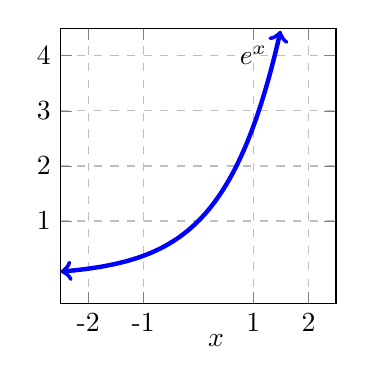
\begin{tikzpicture}[scale=1]
          \begin{axis}[
        %    axis y line = left,
        %    axis x line = bottom,
            xlabel={$x$},
            xtick       = {-2,-1,1,2,3,4},
            xticklabels = {-2,-1,1,2,3,4},
            xlabel style={anchor=west},
            ytick       = {1,2,3,4},
            yticklabels = {1,2,3,4},
            ylabel style={anchor=south},
            samples     = 160,
            domain      = -2:2.5,
            restrict y to domain=-.5:4.5,
            xmin = -2.5, xmax = 2.5,
            ymin = -0.5, ymax = 4.5,
            grid=both, grid style=dashed,
            width=2in, height=2in
          ]
          % pieces 1 and 2
          \addplot[domain=-2.5:2.5, blue, ultra thick, <->] {e^x};
            \node at (1,4) {$e^x$};
        \end{axis}
    \end{tikzpicture}
    \hs{-1.5}\captionof*{figure}{Graph for part (h)}
}{
 \item $\displaystyle\lim_{x\to0^-} \frac{e^x+e^{-x}}{e^x-e^{-x}} $ \\
\blue{
\itemI{
\item The difference between this problem and g) is limit is as $x\to 0^-$ here instead of $x\to \infty$.
\item Every component of $\ds \frac{e^x+e^{-x}}{e^x-e^{-x}} $ is continuous at $x=0$ 
\item As $x\to 0^-$, the numerator $e^x+e^{-x}\to 1+1=2$
\item {\em However} as $x\to 0^-$ in the denominator we have  \\
$\ds \lim_{x\to0^-} e^{x}-e^{-x}\to 1-1=0$ and thus $\ds \frac{e^x+e^{-x}}{e^x-e^{-x}} $ is {\em not } continuous at $x=0$.
\item But we note that the Form is $\displaystyle\lim_{x\to0^-} \frac{e^x+e^{-x}}{e^x-e^{-x}} \to \frac{2}{0}$
\item We need to further decide if From = $\dfrac{2}{0^-}$ or if Form =  $\dfrac{2}{0^+}$
\item $\ds {x\to0^-} $ means we are approaching $0$ from the left, i.e. with values slightly less than $0$.  This means that $e^x$ is slightly {\em less than} $e^0=1$ (see graph on left).  Furthermore, $\ds e^{-x}=\frac{1}{e^x}$ is always  {\em slightly bigger than} $\ds \frac{1}{e^0}=1$. 
\item Thus the denominator $e^x-e^{-x}$ is {\em slightly negative} and thus the Form is $\dfrac{2}{0^-}$
\item All this together means $$\lim_{x\to0^-} \frac{e^x+e^{-x}}{e^x-e^{-x}} \to\frac{2}{0^-}\to -\infty$$
}
}
 }
}



\end{document}
